\chapter{Introduction}
\label{cap1} \vspace{-1cm}

%
%\begin{flushright}
%\begin{minipage}{0.7\linewidth}
%\emph{``Em verdade, em verdade vos digo: quem ouve a minha palavra e
%cr� naquele que me enviou tem a vida eterna, n�o entra em ju�zo, mas
%passou da morte para a vida.''}
%\end{minipage}
%\end{flushright}
%
%\begin{flushright}
%{Jo 5:24}
%\end{flushright}

\section{Motivation}\label{motivation}

In nature it is possible to observe data fusion in a variety of phenomena. Animals combine signals from different senses, such as sight, hearing, smell, taste and touch, to recognize the surroundings. Plants have analogous mechanisms, which are used to modulate water consumption, to change the color of their leaves or to bend their structures towards the light, for instance. Throughout history, the sensory systems in living beings have evolved to assimilate multiple information coming from numerous sources in a highly complex and efficient way, in order to have a better perception of the environment. 

Nowadays information fusion is studied in many fields of science, as a way of exploiting data from multiple sources to achieve better outcomes in comparison to those obtained if any of the sources were used separately \citep{Dasarathy2001}. Other terms have been used to denote the synthesis of information in technical literature, for instance, data fusion, sensor fusion, combination of evidence and synthesis of observations \citep{Goodman1997}. To avoid confusion, the terminology used by \citep{Elmenreich2002} will be adopted, whereby information fusion is understood as the usage of any available information on the system being monitored and sensor fusion is used in cases for which the sources of information are sensor signals. 

Some research fields have been increasingly making use of sensor fusion techniques, such as robotics, biometrics and image processing. The main benefits expected are related to improved \textit{data authenticity}, by increasing accuracy, reliability and confidence, while reducing ambiguity and interference; or \textit{data availability}, with higher spatial and temporal coverages and an increase in the perceived state space dimensionality, that is creating information by combining multiple available data. Consequently much effort has been devoted to developing and investigating data fusion techniques. The work of \citep{Khaleghi2013} presents an extensive review of different available approaches, categorizing them by the way sensor data imperfection is represented, namely, probabilistic fusion, evidential belief reasoning, fuzzy reasoning, possibilistic fusion, rough set-based fusion, random set-based fusion and hybrid fusion. 

Data fusion techniques based on probability theory are the earliest available and perhaps the most popular until now. They are concerned with estimating the probability density functions (PDFs) of the system states by means of the Bayesian approach. If the system is linear and Gaussian, then the Kalman filter (KF) guarantees optimal estimation. For nonlinear processes, KF generalizations were proposed, such as the extended Kalman filter (EKF) or the unscented Kalman filter (UKF) \citep{Julier2004}. On the other hand, particle filters (PF) can be used to deal with both nonlinearities in the dynamics and non-Gaussian distributions \citep{Arulampalam2002}.

The most common class of systems studied in state estimation is the class of sampled-data systems, due to the wide use of digital devices. Although often described by continuous time differential equations, they can be modeled using discrete-time state equations, based on approximation techniques \citep{Phillips1995}. Usually the sampling period of such systems are constant and known. In other words, the sensors are considered to transmit data at regular intervals. However, for many applications, such assumption is not valid. The use of several redundant sensors, for example, with different sampling rates or not synchronized with one another, leads to data being received at irregular instants. Additionally, when data from multiple sensors are transmitted through several subsystems in a network, there might be loss of packets and delays \citep{Schenato2007} or even multiple information arriving simultaneously \citep{Moayedi2011}. In networked control systems, event-triggered sampling schemes have been proposed to optimize the access to communication channels \citep{Hu2017}, which will also generate time-varying sampling intervals. Nowadays, because of the ever-growing scientific advances, the technology of microprocessors, sensors and communication has become increasingly accessible, which continues to ensure that multiple sensor networks are more and more common.

Thus, despite improving accuracy and robustness of the estimation process, the fusion of data from multiple sensors might introduce challenges to the state estimation algorithms, due to sampling irregularities. Depending on how they take place, modifications to the KF and its generalizations can be carried out to tackle these abnormalities. In the work of \citep{Fatehi2017}, the outputs of two individual KFs are fused to estimate the states of a system with multi-rate measurements, whereby one of them is fast, regular and delay-free and the other is slow, irregular and randomly delayed. One application scenario is for industrial process control, where there is online instrumentation characterized by regularly sampled process signals together with asynchronous although very accurate data from laboratory analysis. For a more general case, when the random delays are unknown, the work of  \citep{Gopalakrishnan2010} presents a critical analysis of the available methods for data fusion. They are separated into two categories: those that incorporate the delayed measurements upon arrival, and methods that rely on state augmentation, in order to assimilate the delayed information between estimation steps. 

In general the proposed methods and their performance will depend on the characteristics of the sampling irregularities and how they are modeled. Time delays can be multiples of a base sampling period, for instance. In those cases, delays can happen at single or multiple lags \citep{Penarrocha2012}, they can lead to out-of-sequence measurements \citep{Anxi2005, Westenberger2013} or there can also be data dropouts \citep{Zhu2013}. Nevertheless, the system can be described by a time-invariant discrete-time state equation, with particular representations of the observation model. When measurement are taken after random time intervals, the discrete-time state space representation leads to a time-varying system, since the sampling period changes over time. Some researchers treat the irregular measurement instants as stochastic processes \citep{Micheli2002} or as a periodic sampling interval subject to noisy perturbations \citep{Shen2016}. Generally, the time instant is considered to be the result of a measurement process and the methods assimilate such information in the algorithm, that is the random time intervals are considered as measurements themselves.

To the best of the author's knowledge, no method was proposed so far, for cases in which the random time instants or their statistics are not known or not reliable. If the sampling irregularity is caused due to the lack of sensor synchronization in the network, several algorithms can ensure a common timescale \citep{Sivrikaya2004}, at the expense of additional investments or energy use. Another approach, believed to be largely used in practice, is to simply disregard the irregularities, assimilating the measurements as soon as possible \citep{Kwok2004, Huck2011}. In this case, additional noise will appear in the measurement model as an outcome of not considering the correct time instants. In many cases the statistics of this additional noise is unknown and cannot be accounted for in the estimation process. However, depending on system dynamics and parameters, it might be irrelevant to the overall performance.

Knowing to what extent the estimation accuracy is deteriorated by ignoring the additional uncertainty caused by the sampling irregularity is important to decide whether or not to invest in synchronization. In addition, the investment in more sensors sharing the same network in order to improve accuracy might not pay off, if it increases the occurrence of irregularities. However there are no detailed studies on the behavior of the degradation in accuracy due to neglecting irregularities in the sampling process. Therefore, this work assesses the differences in state estimation performance for systems sampled at random time intervals with and without time-stamp for different scenarios. The purpose is to shed some light on the trade-off for investments in sensor networks and synchronization.

\section{Problem Formulation}\label{sec:problem_form} 

Consider the stochastic nonlinear sampled system
	

\begin{align}
\dot{x}(t) &= f(x(t), u(t), w(t), t),   \label{eq:prob_process} \\ 
y(t_k) &= g(x(t_k) ,v(t_k), t_k), \label{eq:prob_obs}
\end{align}

\noindent
where 	$f\!\!: \mathbb{R}^n \times \mathbb{R}^p \times \mathbb{R}^q \times \mathbb{R^+} \rightarrow \mathbb{R}^n $ and $g\!\!: \mathbb{R}^n \times \mathbb{R}^r \times \mathbb{R^+} \rightarrow \mathbb{R}^m $ are, respectively, the process and observation models, assumed to be known. We assume that for all $k \geq 1$, the observations $y(t_k) \in \mathbb{R}^m$ are available. Process and observation noises, $w(t)$ and $v(t_k)$ respectively, are white, Gaussian, zero-mean and mutually independent, with known covariance matrices. The first two moments of the initial random state vector $x(0)$ are also known. Input data $u(t)$ are available at regularly spaced time intervals $T$, that is $u(iT) \in \mathbb{R}^p$, $\forall i \geq 1$ are known.

Observations are taken at random time instants $t_k$ and are considered to be sorted ($t_{k+1}>t_k,\forall k \in \mathbb{N^+}$) and defined by the time intervals $h_0 \triangleq t_1$, $h_k \triangleq t_k-t_{k-1}, \ \forall k \geq 1$. In this work, we assume that the observation time instants $t_k$ are given by a Poisson random process. In other words, the time intervals $h_k$ are independent and identically distributed (i.i.d.) exponential random variables (RVs) with a known rate parameter $\lambda$, that is $h_k \sim \mathcal{E} (\lambda)$. Since the expected value of an exponential RV is the inverse of its rate parameter, $\lambda$ will sometimes be referred to as expected or average sampling rate of the irregular sampled quantity. An example of time intervals produced by such a random process is illustrated in Figure \ref{fig:amost}. This sampling model characterizes a common application for an event-based sampling scheme or for a networked control system with unsynchronized sensors. \citep{Micheli2002} consider a set of $N$ identical sensors measuring the state variables of a physical process every $L$ seconds. They prove that, if the sensors are independent and unsynchronized and $N$ is large enough, then the waiting time between the realization of two consecutive measurements can be approximated by an exponential random variable $\mathcal{E} (\lambda)$, where the parameter is given by $\lambda = N/L$.

\begin{figure}[h]
	\centering
	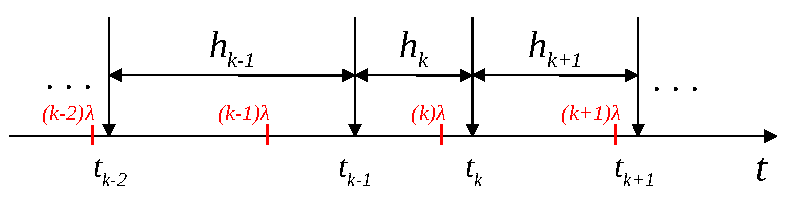
\includegraphics[width=0.8\textwidth]{Imagens/processo_amost.pdf}
	%\setlength{\belowcaptionskip}{-12pt}
	\caption[Irregular sampling process modeled by a Poisson random process]{Irregular sampling process modeled by a Poisson random process. Regularly spaced time intervals $1/\lambda$ are shown in red. An example of time instants $t_k$ realization is also shown, with the respective random time intervals $h_k$. The expected value of time interval is given by $E[h_k]=\frac{1}{\lambda}$.}
	\label{fig:amost}
\end{figure}

%Arrival times to the estimator may be delayed during transmission by a random time amount $\delta_{k}$, also given by exponential random variables, with parameter $\lambda_{\delta_{k}}$, according to Figure~\ref{fig:delay}. Out-of-sequence measurements (OOSM) are not considered in this work. We assume that, in case a measurement delay is so big that its packet arrive later than a future measurement, it gets lost in transmission.
%
%\begin{figure}[h]
%	\centering
%	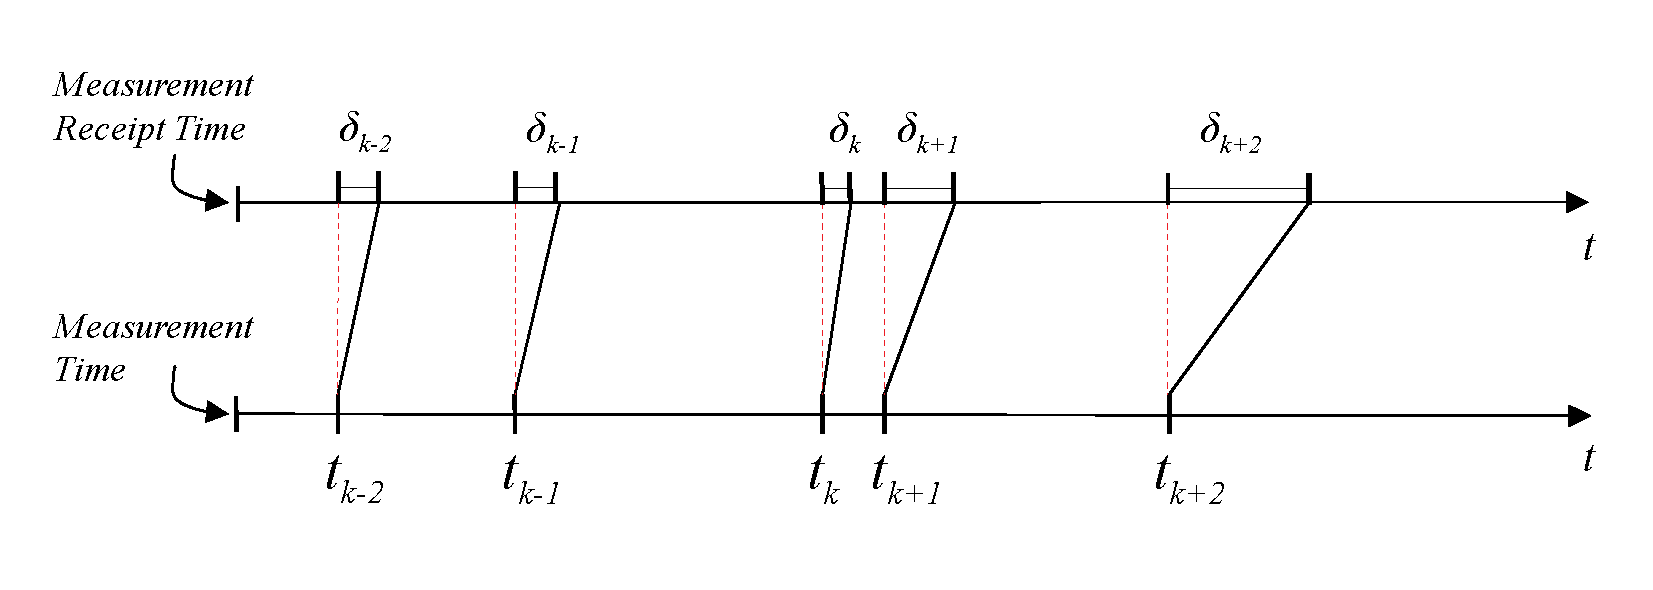
\includegraphics[width=0.8\textwidth]{Imagens/scheme-timedelay.pdf}
%	%\setlength{\belowcaptionskip}{-12pt}
%	\caption[Randomly delayed measurements]{Randomly delayed measurements, modeled as exponential random variables. 	Random measurement times $t_k$ are received by the estimator after a random delay $\delta_{k}$}
%	\label{fig:delay}
%\end{figure}

%\duvida{Como tratar a quest�o do filtro cont�nuo para as entradas u(t)}/

When time-stamp information is available, data assimilation can be performed at the correct measurement instants $t_k$. When they are not, the assimilation moment is considered to be the random receipt time instant or the next estimation moment.

We wish to estimate the state vector $x(t)$ and its covariance recursively, at regularly spaced time intervals $T$, given their initial values $x_0$ and $P_0$, the process (\ref{eq:prob_process})  and observation (\ref{eq:prob_obs}) models, the input or control signals, $u(iT): iT \leq kT$, and the set of past observations, $y(t_k): t_k  \leq kT$. The knowledge of the time intervals $h_{k-1}: t_k \leq kT$ is also taken into consideration when time-stamp information is available. We assume that the average time interval of observations $1/\lambda$ is greater than or equal to $T$ by a factor $\alpha\geq1$, such that $1/\lambda=\alpha T$.

\section{Objectives}\label{objectives}

\todo[inline]{Falta objetivos}
%1 frase para o objetivo geral
%Objetivos espec�ficos

\section{Text Outline}\label{text-outline}
%
This text is organized in six chapters, including this one. Chapter~\ref{cap1} presents an introduction to the object of study, with an overview of the motivations and historical perspective of the theme, objectives and problem formulation.

Chapter~\ref{cap2} presents a review of the sensor fusion field of science, addressing not only the definitions and taxonomy, but also the advantages of combining information from multiple sources. From the four categorization models of the data fusion problem, the one based on data challenges is further explored. We then introduce and discuss the methods proposed in literature to handle imperfect data. 

Chapter~\ref{cap3} discusses the data-related challenges that arise for sampled-data systems, regarding sampling irregularities. Diagrams are built to organize the types, effects and causes of irregularities. We describe the necessary modifications to state estimation observation models, in order to handle such abnormalities in sampling schemes. To perform effective state estimation in the presence of sampling irregularities, methods depend on the knowledge of the exact time measurements were taken. Therefore, we explore time synchronization methods suited for sensor networks.

After the literature review, we focus on the probabilistic sensor fusion approach to sampled-data systems with sampling irregularities. The study of the impact of neglecting time-stamp information is performed.

Chapter~\ref{cap4} describes the methods used for simulation, considering the adaptations for the scenarios with and without time-stamp. We describe the filtering algorithm and the assumptions used for each scenario. Furthermore, we define the performance metrics used for the results assessment.

In Chapter~\ref{cap5} we present simulated results from two systems: an arbitrary linear system and a unicycle position estimation system. Signal parameters are varied to assess the impact in performance of both considering and not considering time-stamp in estimation algorithms. Performance is evaluated using estimated state errors and estimation consistency. 

Finally, we conclude the study in Chapter~\ref{cap6}, highlighting the study limitations and suggestions of future work, apart from evaluating if the proposed objectives were achieved.

\clearpage

%
%\subsubsection{Problema 1: In}\label{sec:entrada_regular}
%
%\textit{As entradas $u(t)$ s�o medidas em intervalos regularmente espa�ados $T$, i.e. $u(iT) \in \mathbb{R}^p$, $\forall i \geq 1$ s�o conhecidas. $w(t) \in \mathbb{R}^q$ � o ru�do de processo. 
%}
%
%\subsubsection{Problema 2: Irregular input sampling}\label{sec:entrada_irregular}
%
%\textit{Medi��es feitas em instantes de tempo aleat�rios $t_{\textrm{u},i}$, $\forall i \in \mathbb{N^+}$, ordenados ($t_{\textrm{u},i+1}>t_{\textrm{u},i}$, $\forall i \in \mathbb{N^+}$) e definidos pelos intervalos de tempo $h_{\textrm{u},0} \triangleq t_{\textrm{u},1}$ e $h_{\textrm{u},i} \triangleq t_{\textrm{u},i}-t_{\textrm{u},i}, \ \forall i \geq 1$. $u(t_{\textrm{u},i}) \in \mathbb{R}^p$, $\forall i \geq 1$ s�o conhecidas. $w(t_{\textrm{u},i}) \in \mathbb{R}^q$ � o ru�do de processo. Assim como para a medi��o irregular da sa�da, os instantes de tempo $t_{\textrm{u},i}$ s�o dados por um processo aleat�rio de Poisson com par�metro $\lambda_u=T$, sendo $T$ o valor esperado do intervalo de tempo $h_{\textrm{u},i}$.
%}
%
%\subsubsection{Problema 2: Irregular sampling with time delay}\label{sec:entrada_irregular}
%\hfill 
%

